% ---------------------------------------------------------------------
\chapter{System and equipment}
% ---------------------------------------------------------------------
Robots are becoming more important in everyday live. Because robots usually work in  a dynamic environments,The robot has to adapt its paths according to the changing environment.For this reason motion planning is an important part for robotics research. In this thesis an algorithm is developed which can create an environment representation suitable for a motion planning algorithm based on point clouds received from a capturing device.
\section{ROS}
ROS (Robot Operating System) is an open source system for operating robots on a computer. A ROS system usually consists of a large number of nodes, any of which can communicate with other nodes in a publish/subscribe manner. As a flexible operating system, the nodes on ROS have great arbitrariness. They can be located on different computers or even on different networks.\\
\begin{figure}[htp]
	\centering % 图片居中
	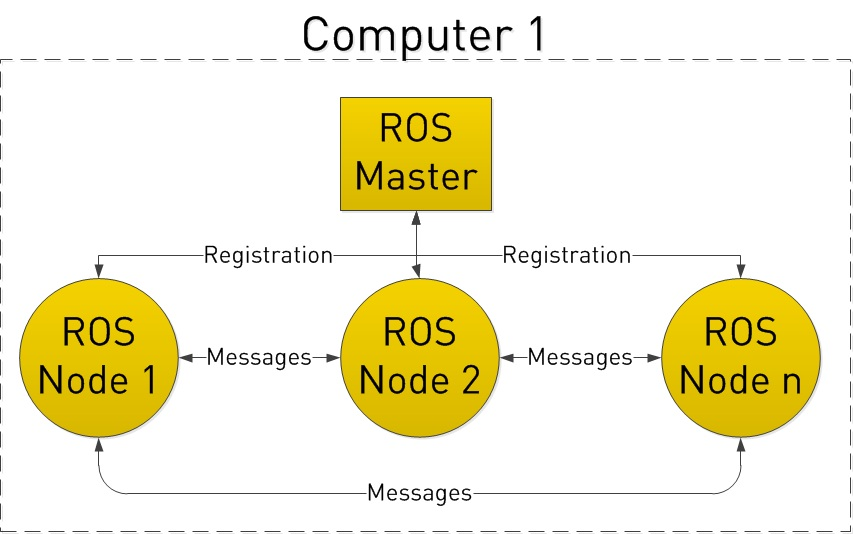
\includegraphics[width = 15.3cm]{figures/Messages}
	\caption{ Messages in ROS}
	\label{fig:figure1label}
\end{figure}
In this algorithm, first we have an administrator (ROS Master) to manage our entire system, and then we need to establish three nodes, namely the camera node, the image processing node in the robot, and the display node on the computer. Then, under the management of ROS Master, the camera node (Camera Node) initiates a session (Topic) to send image information, and at the same time, the other two nodes subscribe to this session (Topic)(For example Figure 2.1). \\
In this way, when the camera node obtains a new image from the camera, it will immediately send the obtained image to the other two nodes (using the network protocol TCP/IP). But if the robot image processing node needs to request information from the camera node at a specific moment, then ROS will use a service request mechanism. First, the image processing node can tell ROS Master that I need to request a service from the camera node, and then ROS Master will establish a service request/response connection channel between the camera node and the image processing node. That is, the image processing node will first request image information, and then the camera node will send the collected information to the image processing node.\\

\section{PCL}
To simplify the handling of point clouds in the algorithms the Point Cloud Library (PCL) will be used. The PCL offers different data types which are used in in this thesis. The PCL also offers a variety of operations which can be performed on the point clouds, e.g. filter operations, segmentation and transformations, which are used especially to prepare the data provided from the capture device for the next step.
\section{D435i}
In this experiment, we used two binocular cameras to obtain point cloud depth information to synthesize objects. We tested several different cameras.
\begin{figure}[htp]
	\centering % 图片居中
	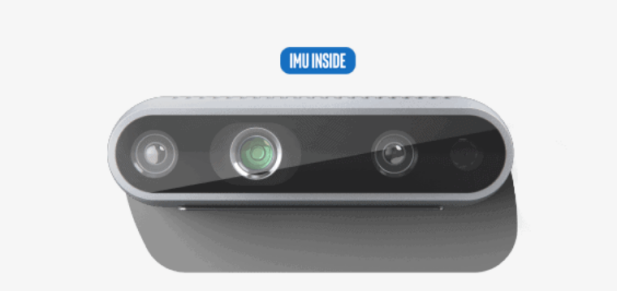
\includegraphics[width = 15.3cm]{figures/camera}
	\caption{ Intel Realsense D435i}
	\label{fig:figure1label}
\end{figure}
-The Intel Realsense SR300 camera uses a structured camera. Each camera emits a light signal of a certain frequency, and then uses the reflection of light to obtain depth information. Therefore, when two cameras work at the same time, light interference will inevitably occur.
-Kinect is a Tof camera and must emit a continuous laser, so there will be interference. In addition, Kinect is too large, which is not conducive to laboratory placement and measurement.
-The principle of RealsenseD455 is binocular stereo vision. Do not rely on reflected light to measure depth information, but the minimum measurement distance is 0.4 meters. The experimental environment we require is less than 0.4 meters, so it is not suitable.
- D435 This kind of camera is a binocular depth camera, it is based on the principle of parallax to obtain the three-dimensional geometric information of the object, and will not actively emit light, so two identical D435 will not interfere with each other. And the minimum measurement distance of D435i is 0.1 meters.
-Realsense D435i has the same principle and structure as D435, but D435i has built-in IMU (D435 has no built-in IMU).
So I chose D435i as the camera for this experiment

